
\documentclass[aspectratio=169]{beamer}

% =========================================================
% THEME
% =========================================================

\usetheme{vub}

% Remove navigation symbols and top black bar
\setbeamertemplate{navigation symbols}{}
\setbeamertemplate{headline}{}



% =========================================================
% PACKAGES
% =========================================================

\usepackage{graphicx}
\usepackage{amsmath}
\usepackage{booktabs}
\usepackage{graphicx}
\usepackage{tikz}
\usepackage{fontenc}
\usepackage{inputenc}
\usepackage{xcolor}
\usepackage{listings}

% ── Colors ──────────────────────────────────────────────
\definecolor{cblue}{HTML}{0EA5E9}
\definecolor{cpurple}{HTML}{8B5CF6}
\definecolor{cgreen}{HTML}{10B981}
\definecolor{cyellow}{HTML}{F59E0B}
\definecolor{cred}{HTML}{EF4444}
\definecolor{cgray}{HTML}{475569}
\definecolor{clightgray}{HTML}{F1F5F9}
\definecolor{ctextgray}{HTML}{334155}
\definecolor{csubtitle}{HTML}{64748B}


% =========================================================
% TITLE PAGE INFO
% =========================================================

\title{Web Wii}

\subtitle{
A Modern Wii Remote Recreation\\
Using IR Tracking and BLE
}

\author{
Mika Baëza \and Mohammad Parto \and Kawtar Bidoukhach
}

\date{SEES Project -- 2026}

% =========================================================



\begin{document}

% =========================================================
% TITLE SLIDE
% =========================================================

\frame{\titlepage}

% =========================================================
% MOTIVATION
% =========================================================

\begin{frame}{Why did we build this project?}
  \vspace{0pt plus 0.3filll}
  \begin{itemize}\setlength\itemsep{0.55em}
    \item Inspired by the Nintendo Wii and its intuitive motion-based interaction
    \item Recreate a modern Wii-like pointing experience
    \item Use embedded hardware for real-time motion tracking
    \item Enable wireless interaction directly through a web browser
  \end{itemize}
  \vspace{0pt plus 1filll}
  \begin{center}
    \large\textbf{Goal:} Create a fully wireless motion-controlled pointing system.
  \end{center}
  \vspace{0pt plus 1filll}
\end{frame}
% =========================================================
% 

% =========================================================
% BACKGROUND
% =========================================================
\begin{frame}{Background: The Original Wii Remote}
  \vspace{0pt plus 0.3filll}
  \begin{itemize}\setlength\itemsep{0.55em}
    \item Wii Remote uses a \textbf{passive IR sensor bar} + on-board camera to track cursor position
    \item Original motion sensing: 3-axis \textbf{accelerometer} --- no rotational tracking
  \end{itemize}
  \vspace{0pt plus 0.8filll}
  \begin{itemize}\setlength\itemsep{0.55em}
    \item We keep the same IR architecture but replace the sensor bar with \textbf{two fixed IR LEDs}
    \item Instead of raw accelerometer data, we use a \textbf{BNO085 IMU} --- outputs Euler angles directly
    \item Orientation is ready to use, no manual sensor fusion needed
  \end{itemize}
  \vspace{0pt plus 1filll}
  \begin{center}
    \large\textbf{Result:} Simpler firmware, more reliable cursor tracking.
  \end{center}
  \vspace{0pt plus 1filll}
\end{frame}
% =========================================================

% =========================================================
% CHALLENGES AND SOLUTIONS
% =========================================================

\begin{frame}{Challenges and Solutions}

\small

\textbf{Challenge 1 — Depth Ambiguity}

\vspace{0.08cm}

When using a single IR point, the controller distance cannot be estimated reliably.

\vspace{0.08cm}

$\blacktriangleright$ \ {\color[rgb]{0.0,0.24,0.45}\textbf{Solution:}} Use two IR LEDs with fixed spacing to recover depth through geometry.

\vspace{0.2cm}

\textbf{Challenge 2 — Orientation Stability}

\vspace{0.08cm}

Raw gyroscope measurements accumulate drift over time.

\vspace{0.08cm}

$\blacktriangleright$ \ {\color[rgb]{0.0,0.24,0.45}\textbf{Solution:}} Use the BNO085 onboard sensor fusion and reset calibration.

\vspace{0.2cm}

\textbf{Challenge 3 — Real-Time Communication}

\vspace{0.08cm}

Cursor updates must remain responsive and low latency.

\vspace{0.08cm}

$\blacktriangleright$ \ {\color[rgb]{0.0,0.24,0.45}\textbf{Solution:}} Use BLE notifications at approximately 100 Hz.

\vspace{0.2cm}

\end{frame}


% SYSTEM ARCHITECTURE
% =========================================================

\begin{frame}

\vspace{0.1cm}

{\Large \textbf{System Architecture}}

\vspace{0.45cm}

\begin{columns}[c]

% ================= LEFT COLUMN =================

\column{0.52\textwidth}

\begin{itemize}\setlength\itemsep{0.55em}
    \item Two IR LEDs are placed near the screen
    \item The remote camera detects the LEDs
    \item The IMU measures controller orientation
    \item The ESP32 computes cursor position
    \item BLE sends cursor data to the webpage
\end{itemize}

\vspace{0.5cm}

\begin{center}
\large\textbf{
IR LEDs $\rightarrow$ Camera $\rightarrow$ ESP32
}
\end{center}

% ================= RIGHT COLUMN =================

\column{0.44\textwidth}

\begin{center}
    \includegraphics[width=\linewidth]{architecture.png}
\end{center}

\end{columns}

\end{frame}

% =========================================================

% =========================================================
% HARDWARE COMPONENTS
% =========================================================

\begin{frame}

\vspace{0.1cm}

\begin{columns}[c]

% ================= LEFT COLUMN =================

\column{0.40\textwidth}

\textbf{Remote Components}

\vspace{0.2cm}

\begin{itemize}\setlength\itemsep{0.5em}
    \item ESP32-S3
    \item BNO085 IMU (UART protocol)
    \item IR Camera (I2C protocol)
    \item Push Buttons
    \item Breadboard Prototype
\end{itemize}

\vspace{0.4cm}

\textbf{Sensor Bar}

\vspace{0.2cm}

\begin{itemize}\setlength\itemsep{0.5em}
    \item 2 IR LEDs
    \item Fixed spacing
\end{itemize}

% ================= RIGHT COLUMN =================

\column{0.56\textwidth}

\begin{center}

% ---------- FIRST ROW ----------

\begin{minipage}{0.45\linewidth}
\centering
\includegraphics[width=0.82\linewidth]{esp32.png}

\vspace{0.08cm}
{\small ESP32-S3}
\end{minipage}
\hspace{0.03\linewidth}
\begin{minipage}{0.45\linewidth}
\centering
\includegraphics[width=0.62\linewidth]{imu.png}

\vspace{0.08cm}
{\small BNO085 IMU}
\end{minipage}

\vspace{0.35cm}

% ---------- SECOND ROW ----------

\begin{minipage}{0.45\linewidth}
\centering
\includegraphics[width=0.72\linewidth]{ircamera.png}

\vspace{0.08cm}
{\small IR Camera}
\end{minipage}
\hspace{0.03\linewidth}
\begin{minipage}{0.45\linewidth}
\centering
\includegraphics[width=0.55\linewidth]{irleds.png}

\vspace{0.08cm}
{\small IR LED}
\end{minipage}

\end{center}

\end{columns}

\end{frame}

% =========================================================

% % % =========================================================
% BNO085 WIRING TO ESP32-S3
% =========================================================

\begin{frame}{BNO085 Wiring to ESP32-S3 (UART-RVC)}

\begin{columns}[c,totalwidth=\textwidth]

% =========================================================
% LEFT SIDE
% =========================================================

\column{0.42\textwidth}

\textbf{Why UART-RVC instead of I2C?}

\vspace{0.25cm}

\begin{itemize}\setlength\itemsep{0.55em}

\item BNO085 I2C is unreliable on ESP32-S3

\item UART-RVC streams orientation continuously

\item Only one wire is needed for data

\item No sensor configuration required

\end{itemize}

\vspace{0.35cm}

\small

{\color[rgb]{1.0,0.35,0.0}\textbf{P0 HIGH}}
enables UART-RVC mode

\vspace{0.08cm}

Baudrate: \texttt{115200}

% =========================================================
% RIGHT SIDE
% =========================================================

\column{0.52\textwidth}

\begin{center}

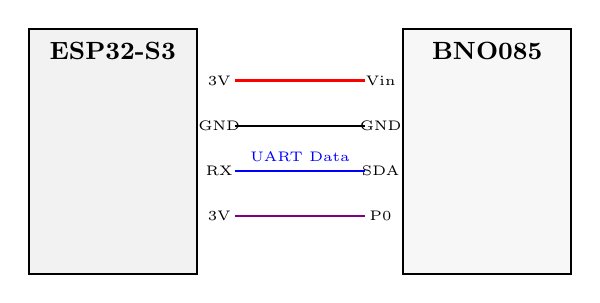
\begin{tikzpicture}[scale=0.82]

% ===== ESP32 =====

\draw[thick, fill=black!5] (0,0) rectangle (2.6,3.8);
\node[font=\bfseries\small] at (1.3,3.45) {ESP32-S3};

% ===== BNO085 =====

\draw[thick, fill=black!3] (5.8,0) rectangle (8.4,3.8);
\node[font=\bfseries\small] at (7.1,3.45) {BNO085};

% ===== Pins =====

\node[font=\tiny] at (2.95,3.0) {3V};
\node[font=\tiny] at (2.95,2.3) {GND};
\node[font=\tiny] at (2.95,1.6) {RX};
\node[font=\tiny] at (2.95,0.9) {3V};

\node[font=\tiny] at (5.45,3.0) {Vin};
\node[font=\tiny] at (5.45,2.3) {GND};
\node[font=\tiny] at (5.45,1.6) {SDA};
\node[font=\tiny] at (5.45,0.9) {P0};

% ===== Wires =====

\draw[red, thick] (3.2,3.0) -- (5.2,3.0);
\draw[black, thick] (3.2,2.3) -- (5.2,2.3);
\draw[blue, thick] (3.2,1.6) -- (5.2,1.6);
\draw[violet, thick] (3.2,0.9) -- (5.2,0.9);

% ===== Labels =====

\node[font=\tiny, above, text=blue] at (4.2,1.6) {UART Data};

\end{tikzpicture}

\end{center}

\end{columns}

\end{frame}


% =========================================================
% HOW THE IR CAMERA WORKS
% =========================================================

\begin{frame}{How the IR Camera Works}

\vspace{0.2cm}

\begin{center}

\includegraphics[
width=\linewidth,
keepaspectratio
]{222.png}

\end{center}

\end{frame}


% =========================================================
% COMPUTATION EXPLANATIONS
% =========================================================

\begin{frame}{Computation overview}

\vspace{-1cm}

\begin{center}

\includegraphics[
width=\paperwidth,
height=0.82\paperheight,
keepaspectratio
]{computation.png}

\end{center}

\end{frame}



% =========================================================
% CURSOR LOCALIZATION PIPELINE
% =========================================================

\begin{frame}{Cursor Localization Pipeline}

\vspace{-1cm}

\begin{center}

\includegraphics[
width=\paperwidth,
height=0.82\paperheight,
keepaspectratio
]{111.png}

\end{center}

\end{frame}

% =========================================================
% COMPUTATION EXPLANATIONS
% =========================================================

\begin{frame}{Computation overview}

\vspace{-1cm}

\begin{center}

\includegraphics[
width=\paperwidth,
height=0.82\paperheight,
keepaspectratio
]{ble_packet.png}

\end{center}

\end{frame}



% =========================================================
% MISS MASK
% =========================================================

\begin{frame}{The \texttt{MISS\_MASK}}

\vspace{0.3cm}

\begin{columns}[c]

% ===== BIT 0 =====

\column{0.31\textwidth}

\fbox{
\parbox[c][2.8cm][c]{0.92\linewidth}{

\centering

{\bfseries Bit 0}

\vspace{0.25cm}

{\large IMU Miss}

\vspace{0.18cm}

\small
BNO085 read failed

}
}

% ===== BIT 1 =====

\column{0.31\textwidth}

\fbox{
\parbox[c][2.8cm][c]{0.92\linewidth}{

\centering

{\bfseries Bit 1}

\vspace{0.25cm}

{\large IR Camera Miss}

\vspace{0.18cm}

\small
IR LEDs not detected

}
}

% ===== BIT 2 =====

\column{0.31\textwidth}

\fbox{
\parbox[c][2.8cm][c]{0.92\linewidth}{

\centering

{\bfseries Bit 2}

\vspace{0.25cm}

{\large Localization Fail}

\vspace{0.18cm}

\small
Invalid 3D estimation

}
}

\end{columns}

\vspace{1cm}

\begin{center}

\small

{\color[rgb]{0.0,0.24,0.45}\texttt{missMask = 0}}
$\rightarrow$
valid packet

\hspace{1cm}

{\color[rgb]{1.0,0.35,0.0}\texttt{missMask $\neq$ 0}}
$\rightarrow$
packet ignored

\end{center}

\end{frame}

% =========================================================



% =========================================================
% WEB INTERFACE
% =========================================================

\begin{frame}{Web Interface}

\begin{columns}[T,totalwidth=\textwidth]

% ================= LEFT COLUMN =================

\column{0.5\textwidth}

\begin{itemize}\setlength\itemsep{0.7em}

\item A browser-based interface was developed using Svelte and SvelteKit

\item The webpage communicates directly with the remote using the Web Bluetooth API

\item Cursor coordinates and button states are updated in real time through BLE communication

\item No native desktop application or driver is required

\item Compatible with Chromium-based browsers such as Chrome and Edge

\end{itemize}

\vspace{0.5cm}

\begin{center}

\small
\texttt{web-wii.couseran.fr}

\end{center}

% ================= RIGHT COLUMN =================

\column{0.45\textwidth}

\centering


\includegraphics[width=0.9\linewidth]{./web_page.png}

\end{columns}

\end{frame}


% =========================================================
% FINAL PROTOTYPE
% =========================================================

\begin{frame}{Final Prototype}

\vspace{0.1cm}

\begin{center}

\includegraphics[
    angle=90,
    width=0.9\textheight,
    keepaspectratio
]{prototype.jpeg}

\end{center}

\end{frame}

% =========================================================
% LIMITATIONS AND FUTURE WORK
% =========================================================

\begin{frame}{Limitations and Future Work}

\begin{itemize}\setlength\itemsep{0.7em}

\item \textbf{IR LED emission angle:}  
The current IR LEDs have a limited emission cone, causing tracking loss when the controller is pointed too far away from the screen axis. Wider-angle IR LEDs could significantly improve robustness.

\item \textbf{BNO085 sensor fusion latency:}  
The onboard fusion algorithm prioritizes orientation stability, introducing a small delay during fast rotational movements.

\item \textbf{Browser compatibility:}  
The system relies on the Web Bluetooth API, which is currently supported mainly by Chromium-based browsers such as Chrome and Edge.

\item \textbf{Future improvements:}  
Potential improvements include wider-angle LEDs, PCB integration for better hardware stability, and software filtering for smoother cursor tracking.

\end{itemize}

\end{frame}

% =========================================================
% CONCLUSION
% =========================================================

\begin{frame}

\vfill

\begin{center}

{\LARGE \color[rgb]{1.0,0.35,0.0}\textbf{Conclusion}}

\vspace{0.6cm}

\parbox{0.82\linewidth}{

\centering

This project successfully recreated the core Nintendo Wii pointing experience using modern embedded hardware, IR tracking, IMU orientation sensing, BLE communication, and browser-based rendering. The final system achieved real-time cursor interaction without requiring native desktop software, while demonstrating that a modern motion-controlled interface can be built using accessible low-cost components and web technologies.

}

\end{center}

\vfill

\end{frame}

% =========================================================
% =========================================================
% THANK YOU SLIDE
% =========================================================


{
\title{{\fontsize{30}{15}\selectfont \bfseries Thank You!}}
\author{}
\date{}
\frame{\titlepage}
}

\end{document}

